\documentclass[10pt,a4paper]{article}
\usepackage[T1]{fontenc}
\usepackage[utf8]{inputenc}
\usepackage{lmodern,microtype,amsmath,amssymb,graphicx,booktabs,tabularx}
\usepackage[a4paper,margin=22mm,top=20mm,bottom=20mm]{geometry}
\usepackage{xcolor,caption,enumitem,fancyhdr,hyperref}
\definecolor{ink}{HTML}{173E41}
\definecolor{link}{HTML}{016B68}
\hypersetup{colorlinks=true,linkcolor=link,urlcolor=link,citecolor=link,pdftitle={When does a fusion tree earn its complexity?},pdfauthor={OKAPI and FusionBench research note}}
\captionsetup{font=small,labelfont=bf,justification=raggedright,singlelinecheck=false}
\pagestyle{fancy}\fancyhf{}\fancyhead[L]{\small\textsf{OKAPI / FusionBench}}
\fancyhead[R]{\small\textsf{Research note}}\fancyfoot[C]{\small\thepage}
\setlength{\headheight}{13pt}
\setlength{\parindent}{1.2em}
\setlength{\emergencystretch}{1.2em}
\renewcommand{\topfraction}{.94}\renewcommand{\textfraction}{.05}
\setlist{nosep,leftmargin=*}
\newcommand{\FB}[2]{\href{https://github.com/damiankucharski/fusionbench/blob/5f9254e0c6e4559d7c0d19f28dc91641fba09d57/docs/ensemble-study/#1}{#2}}
\newcommand{\LAB}[2]{\href{https://github.com/damiankucharski/OKAPI/blob/1d7ad2d1660627585329bc584a9c4634915e8bb1/#1}{#2}}
\begin{document}
\thispagestyle{empty}
\noindent{\sffamily\small\color{ink}{OKAPI / FUSIONBENCH}\hfill 28 NOVEMBER 2026}\par
\vspace{1em}
{\noindent\sffamily\bfseries\fontsize{26}{30}\selectfont When does a fusion tree\\earn its complexity?\par}
\vspace{.5em}
{\noindent\large A research note on learning, selecting and interpreting ensembles of predictions\par}
\vspace{.85em}\hrule\vspace{.8em}
\noindent\textbf{Abstract.}
A fusion tree can express a good rule, fail to discover it, or discover it and lose it during selection. We study these failure modes separately using controlled prediction banks, native OKAPI program replays and external classification tasks. On a fixed panel of 24 FusionBench scenarios, a validation-selected tree combining derivative-free logit fitting with genetic programming achieved mean test Brier loss .21456 versus .24431 for probability logistic stacking. The GP candidate alone scored .28419. On a controlled null, noisy evolution discarded an explicitly seeded optimal program in all twelve banks. A conservative replacement rule prevented harmful moves, yet could not accept a supplied true improvement on any of 48 signal banks. Matched controls and counterexamples identify what justifies a library feature and what still requires experimental development.

\section{Experimental contract}
A prediction bank contains $M$ providers' class probabilities for the same observations, together with their labels. A fusion algorithm sees provider outputs. A network predicting from original observations requires access to those inputs at deployment. FusionBench supplies reproducible laws over predictions and labels. Controlled changes can vary provider competence, redundancy, class confusion, dependence or transfer between development and test. The suite grew from 19 scenarios to 20 with a predefined similar-classes task and subsequently to 24. \FB{scenario-coverage/README.md}{Scenario coverage.} \FB{external-coverage/README.md}{External checks.}

Our primary metric is full-class Brier loss, $L(p,y)=\sum_{c=1}^{C}(p_c-\mathbf{1}\{y=c\})^2$, averaged over observations. For binary probabilities it equals twice the positive-class squared error. Earlier studies reporting the latter are identified below. The matched panel includes three inexpensive references:
\begin{itemize}
\item \textbf{Mean} averages every provider's probabilities with no fitted parameters.
\item \textbf{Ranked-prefix Top-$N$} ranks individual providers by development Brier, evaluates the mean of each successive prefix and selects the best prefix on development labels.
\item \textbf{Probability LR} is regularized logistic stacking on standardized probability features (regression $C=1$). A second reference uses logits. Multiclass stacking can learn effects across class columns. Learning a combiner on held-out provider outputs follows the stacked generalization literature \cite{ting}.
\end{itemize}
The principal replay uses 24 fixed scenarios, six independently seeded banks per scenario, 640 development and 1,024 test rows per bank. Methods share observations and labels. Test outcomes are used only after selection. Each scenario contributes equally. Paired intervals resample banks within each scenario, conditioning on these 24 scenarios. Overlapping real-data splits and generator families selected during benchmark development limit extrapolation. \FB{replacement-experiment/panel/protocol.md}{Design.} \FB{replacement-experiment/panel/results/banks.json}{Bank fingerprints.}

\section{A learnable native tree}
For binary inputs $p_m$, a native head predicts $\sigma(a+\sum_m w_m\,\operatorname{logit}(p_m))$, with clipped inputs before taking logs. An input can be the output of a whole evolved subtree. A negative coefficient can correct shared noise even for individually calibrated providers \cite{kahn}. In the shared-weight multiclass head the corresponding class score is $\sum_m w_m\log p_{mc}$, normalized over classes. Deterministic local parameter search accepts a caller's scalar fitness, including objectives without gradients. Joint structure search and local parameter tuning also have precedents in symbolic regression \cite{kommenda}. Screening the archive tests up to three novel, non-singleton programs for incremental fitness using signed trial coefficients. The selected programs can receive new weights during joint fitting. \LAB{okapi/pattern_logit.py}{Fitter.} \LAB{okapi/pattern_features.py}{Screening.}

Writing $z_m$ for log evidence (class-centered in the multiclass variance estimate), the tested fit maximizes an empirical score minus
\[
 \frac{\lambda}{n}\sum_m w_m^2\,\widehat{\mathrm{Var}}(z_m).
\]
The intercept is unpenalized. The experiment fixed $\lambda=.25$. In a 19-family confirmation panel with ten fresh banks per family, this penalty moved primary Brier from .21524 to .20673 (difference $-.00851$, 95\% interval $[-.01079,-.00624]$). That score mixes clean test, independent logit perturbations and one provider supplying another example's predictions with weights $.50/.25/.25$. Handcrafted pairwise minima in a separate ablation gave $-.00069$ with an interval spanning zero. \FB{pattern-iterations/README.md}{Ablations and controls.}

In the 24-scenario replay, GP explores on 448 discovery rows for 600 scoring visits. On the remaining 192 rows the procedure chooses between a provider-only head, a head augmented with selected GP features, and a GP tree. A selected head is refitted on all development rows with the structure fixed. A deployed tree can still require multiple providers. Table~\ref{tab:panel} distinguishes the full procedure from a component and a short search. \FB{replacement-experiment/panel/compare_variants.py}{Matched replay.}

\begin{table}[htbp]\centering\small
\caption{Test Brier on identical banks. The GP-only row deploys the longer procedure's GP candidate on every bank. The short search offers 72 offspring. Proposal counts and scoring visits measure different work.}\label{tab:panel}
\begin{tabularx}{.98\linewidth}{@{}Xr@{}}\toprule
Procedure & Mean test loss\\\midrule
Mean of all providers & .37756\\
Best development-ranked prefix & .33838\\
Logistic stacking, probabilities & .24431\\
Logistic stacking, logits & .24744\\\addlinespace
Longer native procedure, GP candidate alone & .28419\\
Longer native procedure, validation-selected tree & \textbf{.21456}\\\addlinespace
Short ordinary GP, all development rows for discovery & .35892\\
Short GP, open breeding and empirical replacement & .36252\\
Short GP, open breeding and certified replacement & .44686\\\bottomrule
\end{tabularx}
\end{table}

The selected tree beat probability LR on 18 of 24 scenario means, by .02976 Brier on average (native minus LR, 95\% interval $[-.03165,-.02785]$). Validation chose the augmented head 77 times, the flat head 40 times and the GP candidate 27 times. Figure~\ref{fig:panel} shows the six reversals. On six different earlier seeds per scenario the corresponding macro scores were .21408 and .24545. These comparisons cannot separately identify the effects of initialization, family selection and search budget. They also cannot predict the performance of stock OKAPI under its defaults. \FB{replacement-experiment/panel/README.md}{Comparisons and costs.}

\begin{figure}[!t]\centering
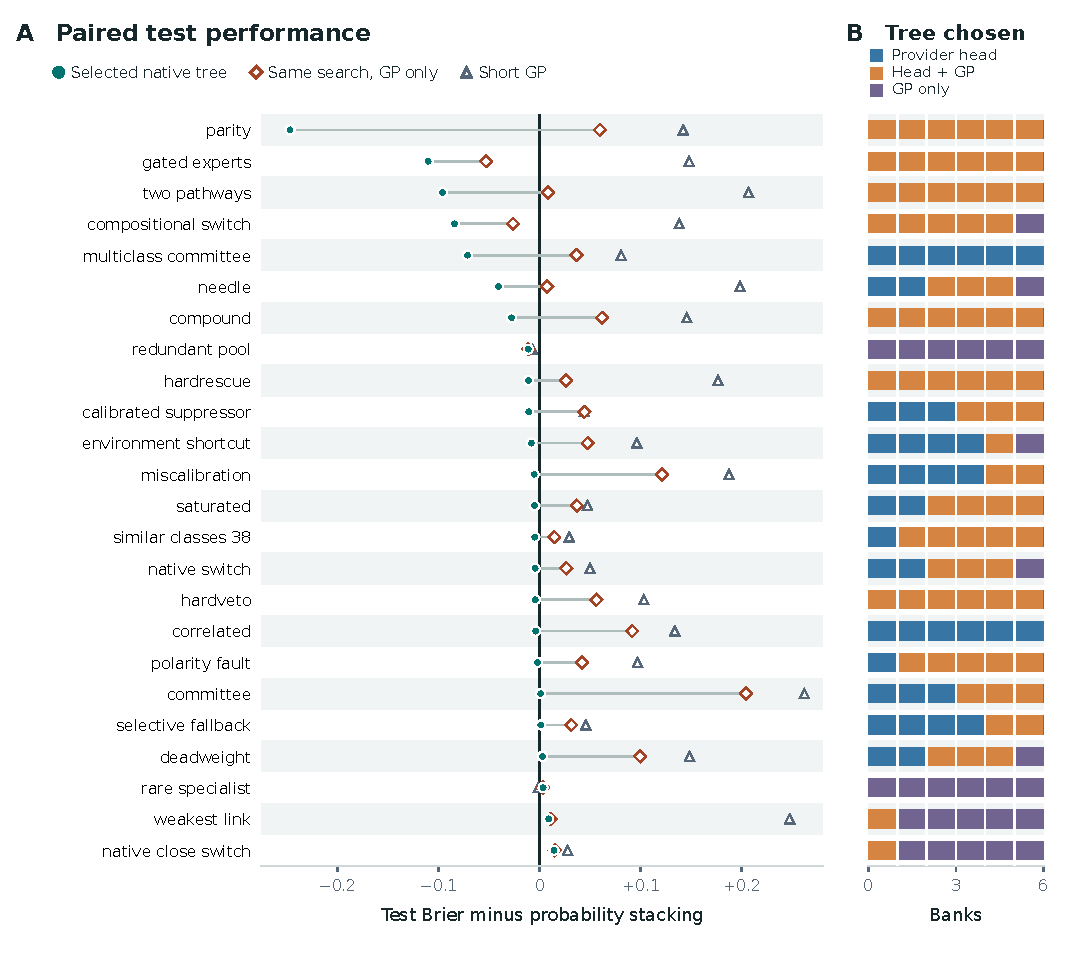
\includegraphics[width=.96\linewidth]{figures/native-performance.pdf}
\caption{Each point averages six paired test differences for one scenario. Negative values favor the indicated procedure over probability LR. Right: counts of the three families selected on validation. Short GP and the longer procedure's GP-only candidate show why the choice of training and deployment procedure changes the comparison.}\label{fig:panel}
\end{figure}

\subsection{Class identities can help a stacker}
With three providers and ten classes, an own-class regression has 30 slope coefficients and ten intercepts. Unrestricted regression has 300 and ten, respectively. These counts describe the parameterization before identifiability constraints. It can use the probability assigned to class 8 to help score class 3. On the same digits bank (logistic regression, nearest neighbors and random forest), full stacking scored .03190, own-class stacking .03402, and the earlier native procedure .03868. A native full affine node replayed the production stacker's coefficients within $8.4\times10^{-8}$ across 72 banks. Fitting its own weights attained .03597 on this digits pool. On another digits pool full LR scored .03616 versus .03287 for own-class LR. The representation can reproduce the stacker, while the learned rule and the benefit of capacity depend on the data. The two pools also used different splits.

The controlled similar-classes experiment varies a shared preference for a wrong destination class and each provider's private preferences, preserving the correct-class probability and each provider's sorted probabilities. With private destinations, unrestricted LR improved Brier by .00439 on the affected classes relative to own-class LR, yet the gain over all classes was only .00032. With the shared pair, the overall comparison favored own-class LR by .00077. Off-diagonal coefficients can encode real class structure. The digits observations alone do not identify a particular pair as its cause. \FB{class-capacity/README.md}{Real pools and paired interventions.}

\section{What a tree search can find, explain, and compile}
\label{sec:mechanism-history}

\subsection{Separating an inaccessible rule from a poor rule}

For binary providers with identity postprocessing, thresholding a tree built
from MIN and MAX turns its gates into AND and OR. The sets of providers above
threshold on which the tree is positive form an upward-closed family.
Conversely, taking the maximum over the minima of its minimal accepted sets
constructs an attaining tree. Sorting each observation's provider scores
expresses its squared loss as a sum of increments on those sets. One minimum
cut therefore gives an exact empirical optimum over \emph{all sizes} for this
grammar. Eight providers require 256 subset vertices. On a two-pathway problem
with 128 fit labels, the exact fit winner reached .09732 IID positive-class
Brier, native GP .21254, arithmetic averaging .15528, ranked-prefix Top-$N$
.16191, and logistic stacking .13997. Under the prespecified detector shift,
the exact winner's advantage over stacking fell from .04265 to .00176.
The certificate concerns empirical optimization within the stated grammar.
\href{https://github.com/damiankucharski/fusionbench/blob/1f12dbf/docs/ensemble-study/search-regret/continuous.md}{Cut construction, data and population controls.}

The obstruction was observable in actual populations. On a separate
four-provider problem the empirical optimum equalled the generating rule in
all 12 banks, yet neither rounded nor unrounded GP found it in 24 starts per
precision at 400 evaluations. At generation 15 in a further experiment,
exhausting the legal parent and physical swap choices in 32 populations found
zero next crossovers capable of producing the two-pathway target. On eight
anonymous inputs, changing the initial topology while matching tree size,
inputs and operators increased exact recoveries from 11/24 chain starts to
21/24 branched starts. Only one branched start already contained the answer.
Twelve of the twenty later branched discoveries had a productive crossover
available at initialization. The other eight required intervening changes.
The same topology comparison on the fixed 19-scenario suite gave a full-class
IID Brier difference of $+.00044$ (paired 95\% interval
$[-.00286,.00374]$).
\href{https://github.com/damiankucharski/fusionbench/blob/fbeae0d/docs/ensemble-study/selection-precision/README.md}{Exact search and precision.}
\href{https://github.com/damiankucharski/fusionbench/blob/31466b1/docs/ensemble-study/semantic-donors/README.md}{Legal-swap enumeration.}
\href{https://github.com/damiankucharski/fusionbench/blob/d79f228/docs/ensemble-study/seed-geometry/README.md}{Matched starters and transfer.}
\href{https://github.com/damiankucharski/OKAPI/blob/47029ef/experiments/initial_crossover/README.md}{Independent native crossover replay.}

\subsection{Which operator changes matter?}

Replacing an existing operator family while preserving its ordered arguments
tested a point mutation previously deferred in OKAPI. Enabling the native
extension moved mean full-class IID Brier from .26839 to .25947 across 19
scenarios. Stacking reached .22874. On fresh banks a fourth mutation
opportunity returned either the actual retyped tree or its unchanged
genotype, while consuming the same proposal randomness at that event.
Retyping improved Brier by .01202 relative to this control at 1,200 fitness
evaluations (95\% interval $.00648$--$.01756$). On the nine registered shifts
the interval included zero. A separate structural-identity repair stopped
different programs being merged merely because their printed node sequences
matched. In 48 matched MIN/MAX runs it changed five search paths at 300 calls
and changed none of the selected winners. Correct identities matter even when
a bounded search does not improve.
\href{https://github.com/damiankucharski/fusionbench/blob/d4c4bd1/docs/ensemble-study/full-suite-point/README.md}{Registered suite.}
\href{https://github.com/damiankucharski/fusionbench/blob/b93281d/docs/ensemble-study/mutation-opportunity/README.md}{Slot-matched controls.}
\href{https://github.com/damiankucharski/fusionbench/blob/949ec0d/docs/ensemble-study/search-regret/structural-key/README.md}{Collision replay against the empirical optimum.}

An operator's frequency does not establish its predictive contribution. In a
12-seed rescue circuit, retaining a MAX update repaired 857 decisions and
introduced 168 errors per 8,192 held-out examples on average, relative to
bypassing the update. Duplicating the update kept the
function unchanged and made either single bypass have zero effect. A joint
bypass recovered the original effect for the same operand order. In a
separate switching experiment the algorithm recorded ancestry, then bypassed
all genuinely inherited occurrences in each frozen winner. On the FAR law,
excess positive-class Brier rose from .00267 intact to .02437 on fresh data.
Resetting just the inherited cutoffs gave .01382. Together these interventions
locate the operation and parameter responsible for the measured change.
\href{https://github.com/damiankucharski/OKAPI/blob/9d06b7a/experiments/README.md}{Duplicate intervention and operand order.}
\href{https://github.com/damiankucharski/fusionbench/blob/eea68d5/docs/ensemble-study/search-regret/gate-necessity/README.md}{Inheritance, bypass and reset.}

\subsection{When one network can replace the ensemble}

A binary sigmoid expert with known affine logit on a shared raw input can be
inlined into a circuit. Monotonicity moves the final sigmoid outside a MIN/MAX
tree, and $\max(a,b)=b+\mathrm{ReLU}(a-b)$ implements each binary maximum
(with the analogous identity for minimum). Eight compiled GP trees reproduced
their probabilities within $5.56\times10^{-16}$ on 4,096 held-out rows per
tree. Only one of the 17 natural binary gates disappeared. Their accuracy
remained 84.86\%, while the known median of the same local experts achieved
98.45\%. This route needs the local affine maps and the same coordinates at
deployment. With opaque providers, a small fusion circuit can still require
all of their predictions. For example, 66 ReLUs exactly average 10,395
perfect-matching trees on 12 provider scores when exactly two or three
inputs are high. A fourth high input can activate two disjoint pairs and
cause double counting. On eight inputs with a uniform matching prior the
pair-only formula then gives $6/7$ where the true value is $27/35$.
\href{https://github.com/damiankucharski/OKAPI/blob/35ca8e6/okapi/lattice.py}{Native compiler.}
\href{https://github.com/damiankucharski/fusionbench/blob/d10b51e/docs/ensemble-study/lattice-compile/README.md}{Prediction and gate replay.}
\href{https://github.com/damiankucharski/fusionbench/blob/8f0ba19/docs/ensemble-study/search-regret/matching-compression/README.md}{Exact mixture, counterexample and higher-order correction.}

Recovery from raw observations depends on whether the latent axes can be identified. On
two-pathway data, estimating axes from 4,096 unlabeled mixtures by independent
component analysis and choosing a signed read-once circuit with 32 task
labels reached 93.5\% accuracy across twelve rotated bimodal problems,
against 79.4\% for an MLP. Replacing the latent factors by isotropic Gaussians
with matched covariance made all rotations equally consistent with the unlabeled distribution. Circuit
accuracy fell to 66.6\%, against 72.4\% for the MLP. An out-of-family XOR target also exposed the imposed grammar: with 128
labels, the read-once circuit reached 71.1\% versus 94.4\% for a sign-table
lookup.
\href{https://github.com/damiankucharski/fusionbench/blob/55de703/docs/ensemble-study/README.md}{Blind reconstruction, label budgets and XOR control.}

\paragraph{Further checks for reconstruction.}
Three other lines delimit what can be inferred from recorded predictions.
First, two individually calibrated providers can require a \emph{negative}
logit coefficient when they share class-conditional noise. A signed stack
scored .08481 against .11304 for nonnegative slopes in 24 banks.
Second, the extreme consistent rules in the full noiseless monotone Boolean
class give a minimax midpoint with positive-class Brier $D/4$ on disagreement
mass $D$. Four candidate coordinate projections break the required closure.
Third, estimating a target context mixture improved frozen-tree selection by
.01479 Brier when within-context labels stayed stable, but worsened it by
.02754 when labels reversed with identical observed target predictions.
These give concrete checks on slope constraints, feasible function classes
and access to target labels.
\href{https://github.com/damiankucharski/fusionbench/blob/62afd10/docs/ensemble-study/calibrated-suppressor/README.md}{Signed pooling.}
\href{https://github.com/damiankucharski/fusionbench/blob/d4b9c98/docs/ensemble-study/monotone-envelope/README.md}{Extremal rules.}
\href{https://github.com/damiankucharski/fusionbench/blob/e529e8c/docs/ensemble-study/frozen-pair-ranking/README.md}{Observable drift and silent reversal.}

The linked extensions test whether a purported reference copies its input,
how paid labels expose silent failures, and whether fewer fusion operations
save actual provider calls or wall time. On 16 focal pruned trees only two
dropped a provider. An exact softmax router was slower than the full pool at
batch size one in all twelve tested layouts.
\href{https://github.com/damiankucharski/fusionbench/blob/27edd41/docs/ensemble-study/reference-copy/README.md}{Reference-copy ambiguity.}
\href{https://github.com/damiankucharski/OKAPI/blob/3f64a16/experiments/paired_label_audit/README.md}{Paired label auditing.}
\href{https://github.com/damiankucharski/fusionbench/blob/9af5f79/docs/ensemble-study/prune-frozen-mix/README.md}{Pruning and provider counts.}
\href{https://github.com/damiankucharski/fusionbench/blob/2204351/docs/ensemble-study/softmax-routing/README.md}{Decision routing and timings.}


\section{Where validation overfitting enters}
\textbf{Selection and candidate loss.}
The optimizer's curse arises when selecting a winner among noisy estimates favors positive estimation errors. It can affect the final decision and the set of candidates that reach it \cite{cawley}. In 144 banks the selected tree's apparent Brier gain over the mean was .16914 on internal validation and .16223 on an independent same-law audit. A terminal holdout has a measurable cost: using 448 rather than 640 fit rows lost .00586 on the source audit, and reranking the frozen candidates on the other 192 rows recovered .00417. \FB{validation-curse/README.md}{Split accounting and audit.}

The simulator lets us integrate out test-label noise using the known posterior. With 24 independent training units and eight correlated annotations per unit, ordinary GP's final empirical winner had excess Brier .05816. A hindsight oracle over its last population still had excess .04773. A second experiment explicitly seeded the optimal mean at initialization. All twelve ordinary searches had lost every equivalent survivor by generation four. Evaluating conditional expected training loss on the same training inputs preserved the mean in all twelve final populations. This control requires the simulator's posterior. A group-aware uncertainty penalty helped in the constructed null, yet hurt the informative-provider control. On the full panel subtracting one estimated standard error of improvement during search moved .21408 to .21606 ($+.00198$, interval $[+.00042,+.00354]$). \FB{validation-curse/grouped/README.md}{Population trajectories.} \FB{validation-curse/panel/round2/README.md}{Panel intervention.}

\textbf{Why anchoring the training objective can change the tree.}
For prior $b$, candidate $T$ and positive tree share $t$, deploy $b+t(T-b)$. Under full-class Brier define $H_T=\mathbb E\langle Y-b,T-b\rangle$ and $D_T=\mathbb E\|T-b\|^2$. Expanding the square gives the gain over the prior:
\[
G_t(T)=2t H_T-t^2 D_T.
\]
On a fixed fit sample and finite menu, division by $t$ shows that lowering $t$ reduces the penalty on raw displacement $D_T$. The two optimality inequalities at $t_1<t_2$ give $(t_2-t_1)(D_{T_1}-D_{T_2})\ge0$. In 192 banks the training winner changed 122 times when selected inside the mixture. Every changed winner moved farther from the prior on fit. Deployed with the same $t=.25$, the paired test difference was $+.00069$ (interval $[-.00132,+.00276]$). Whether a farther correction captures noise or signal determines its test value. \FB{anchoring-geometry/README.md}{Derivation and exact finite counterexample.}

Kucharski's dissertation reports a related pattern at prior weight .85. On STARCOP, in-search mixing achieved F1 .7537 on validation and .6996 on test, versus .7497 and .7020 for mixing after selection. On MedMNISTv2, test PR-AUC was .8054 and .8056 respectively, compared with .8047 for the 30-provider mean. A sparse correction still needed all 30 prior providers at deployment. These figures come from the original tables. Individual scene and patient predictions were unavailable for reanalysis. The Brier identity does not give an F1 or average-precision guarantee. \href{https://bip.polsl.pl/wp-content/uploads/sites/4/2026/11/Damian-Kucharski_rozprawa-doktorska.pdf\#page=124}{Dissertation, Sections 5.7 and 6.3.}

\textbf{A separate issue with Pareto truncation.}
In a pooled binary confusion table F1 is determined by precision and recall. Appending F1 can change the order of nondominated points by distance to the ideal even when the front is unchanged. A two-candidate native replay exhibits this reversal. The noisy-survival witness already occurs with one predictive objective and size. The example motivates studying survivor ranking with controlled candidates. Whether additional objectives caused the real-data overfit remains open. \FB{anchoring-geometry/replacement-and-pareto.md}{Worked Pareto example.}

\section{Can we test a replacement before deploying it?}
Each generation proposes twelve children. An incumbent changes only when a child's paired Brier improvement has a positive lower bound on a fresh block of independent labels. The bound uses rowwise possible gains, rescales them to $[0,1]$, and inverts a one-sided Bernoulli KL inequality. A total error budget .05 is allocated across twelve slots and six stages. This controls false certifications conditional on those inputs and the past. Distribution shift falls outside the guarantee. Open breeding permits an unconfirmed program to reproduce. Strict breeding also applies the test to admission. \FB{replacement-experiment/protocol.md}{Derivation and protocol.}

Three providers on eight equally likely input configurations provide a direct power check. In the null law the posterior equals their mean. In the signal law it equals $\min(C,\max(A,B))$ after a randomized assignment of provider roles. The exact solution improves population Brier by $9/64$. When handed directly to the confirmation step, empirical promotion accepted it on 48/48 blocks and certified promotion on 0/48. Even the most favorable possible labels on each of those specific 128-row blocks could not clear the bound. The same certificate protected the optimal incumbent on every null bank. A successful null control alone would have recommended a rule with virtually no power here. \FB{replacement-experiment/controlled/README.md}{Matched laws and attainable-bound calculation.}

On a planted XOR route, two neutral subtrees compose via MAX to yield the exact posterior. With intermediates supplied, open breeding deployed the exact result 30/32 times and strict breeding 0/32. Without supplying the route, neither search proposed an exact solution in any of the 32 banks (Fig.~\ref{fig:mechanisms}). On the 24-scenario suite the two open arms followed identical proposal paths. Certified replacement worsened test Brier by .08434 (interval $[+.06123,+.10481]$) relative to empirical replacement and retained the initial singleton on 140/144 banks. This isolates a failure of the replacement decision at the available budget. Keeping a neutral structure alive and finding it through ordinary variation merit separate controls. \FB{replacement-experiment/barrier/README.md}{Supplied and organic XOR.} \FB{replacement-experiment/panel/README.md}{Matched panel.}

\begin{figure}[htbp]\centering
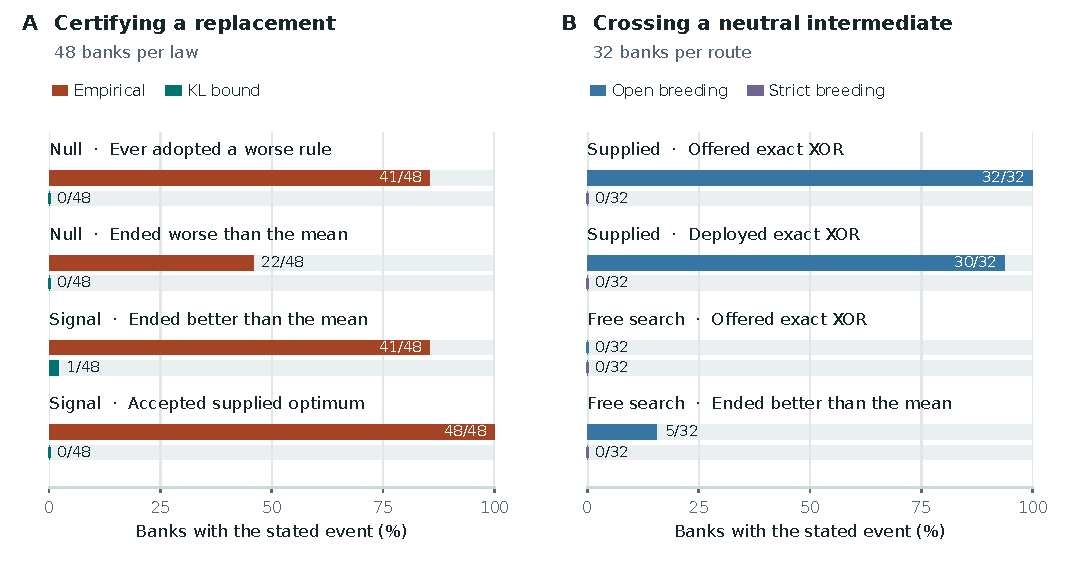
\includegraphics[width=\linewidth]{figures/replacement-mechanisms.pdf}
\caption{Counts across matched banks. Panel A compares empirical and certified promotion on the mean-optimal null and on a nonlinear signal. Panel B compares open and strict certified breeding when the neutral XOR intermediates are supplied or have to be discovered. Each panel names its denominator.}\label{fig:mechanisms}
\end{figure}

\section{What belongs in the library?}
Two independently callable components have an established use and a testable contract: fitting signed native logit weights to a caller's objective, and screening archived programs for complementary features. They operate on existing trees and support evaluation with fresh provider predictions. The reviewed library change exposes both as opt-in primitives. Reproducing Table~\ref{tab:panel} also requires the pinned FusionBench discovery, validation and refitting protocol. The benchmark orchestration and simulator oracles remain in the research repositories. The controlled replacement rule, global uncertainty penalty, alternate initial populations and unrestricted cross-class nodes have informative failure cases or unresolved transfer. The evidence index retains those implementations and results.

Two experiments would distinguish the leading uncertainties. First, predeclare a replacement criterion that has measurable power on a supplied true program at realistic label budgets, then freeze it before testing new null banks and the full suite. Second, freeze a native fitting and family-selection protocol and take it to fresh real prediction banks, separating independent cases or acquisition groups before choosing the rule. Report the mean, ranked-prefix average and probability stacking on the same splits, together with the number of provider calls needed by the deployed tree.

\paragraph{Reproducibility.} The companion \href{https://github.com/damiankucharski/OKAPI/blob/review/native-logit-fitting-and-research-note/docs/research/ensemble-fusion/evidence.md}{evidence index} groups the archived investigations by question, including negative results and counterexamples. Its links identify pinned data, source, protocols and historical literature. The figures are computed from frozen CSV files. Commands accompany the \href{https://github.com/damiankucharski/OKAPI/blob/review/native-logit-fitting-and-research-note/docs/research/ensemble-fusion/index.md}{article source}.

\begin{thebibliography}{9}\small
\bibitem{ting} K.\,M. Ting and I.\,H. Witten (1999). Issues in stacked generalization. \textit{Journal of Artificial Intelligence Research} 10, 271--289. \href{https://doi.org/10.1613/jair.594}{Article.}
\bibitem{kahn} J.\,M. Kahn (2004). A generative Bayesian model for aggregating experts' probabilities. \textit{Proceedings of UAI}, 301--308. \href{https://arxiv.org/abs/1207.4144}{Article.}
\bibitem{kommenda} M. Kommenda, B. Burlacu, G. Kronberger and M. Affenzeller (2020). Parameter identification for symbolic regression using nonlinear least squares. \textit{Genetic Programming and Evolvable Machines} 21, 471--501. \href{https://doi.org/10.1007/s10710-019-09371-3}{Article.}
\bibitem{cawley} G.\,C. Cawley and N.\,L.\,C. Talbot (2010). On over-fitting in model selection and subsequent selection bias in performance evaluation. \textit{Journal of Machine Learning Research} 11, 2079--2107. \href{https://www.jmlr.org/papers/v11/cawley10a.html}{Article.}
\end{thebibliography}
\end{document}
